\section{Metody kompensacji dyspersji}

Wszystkie zaimplementowane metody związane z kompensacją dyspersji znajdują się w pliku $compensation\_disp.py$ w folderze Propagation. Lokalizację pliku przedstawia rysunek \ref{fig:compensation}
\begin{figure}[h]
\centering
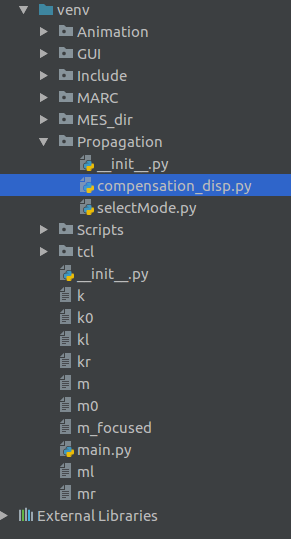
\includegraphics[width=8cm]{Zdjecia/5/kasia/compensation}
\caption{Lokalizacja pliku $compensation\_disp.py$ w drzewie projektu}
\label{fig:compensation}
\end{figure}

Trzy podstawowe metody znajdujące się w tym pliku odpowiadają trzem opisanym wcześniej metodom kompensacji. Są to:

$linear\_mapping\_compensation(signal, number\_of\_modes, disp\_curves)$ funkcja kompensująca dyspersję przy pomocy liniowego przybliżenia szeregu Taylora, opisana w rozdziale 4.4. Funckja przyjmuje trzy argumenty. Pierwszy z nich , $signal$, jest dwuelementową tablicą reprezentującą sygnał, który ma zostać skompensowany. $signal[0]$ to wektor czasu tego sygnału, natomiast $signal[1]$ to wektor wartości sygnału w kolejnych chwilach czasowych. Konwencja przechowywania sygnału w postaci dwuelementowej tablicy jest zachowana w calym pliku. Kolejnym przyjmowanym argumentem, $number\_of\_modes$, jest to liczba całkowita, będąca indeksem krzywej dyspersji, która powinna zostać użyta do kompensacji dyspersji. ostatnim argumentem, $disp\_curves$, jest obiekt klasy $SelectedMode$ przechowującym zaagregowane krzywe dyspersji. wartością zwracaną jest skompensowany sygnał w postaci dwuelementowej tablicy $[wektor\_czasu, wektor\_wartości]$.

$time\_reverse\_compensation(signal, distance, numbers\_of\_modes, disp\_curves)$ funckja generująca sygnał, którego zadaniem jest skompensowanie się na zadanej odległości przy założeniu propagacji wybranych trybów fali. Metoda ta opisana została w rozdziale 4.3. Funkcja przyjmuje cztery parametry. Pierwszy z nich, $signal$ jest sygnałem, który użytkownik chce otrzymać po propagacji. Jego format jest analogiczny jak w poprzednio omawianej funkcji. Kolejny argumentem jest $distance$. Jest to liczba, wyrażająca w metrach odległość po jakiej sygnał powinien się skompensować. Następny argument to $numbers\_of\_modes$. Jest to jednowymiarowa tablica liczb całkowitych. Zawiera ona indeksy krzywych dyspersji, tych postaci fali, które mają propagować w pręcie. Funckja zwraca sygnał, który przepropagowany przez pręt, o zadaną odległość sam się skompensuje. Ostatnim argumentem jest obiekt przechowujący krzywe dyspersji.

$mapping\_from\_time\_to\_distance(dispersion, dispercion\_curves,$
$ propagated\_modes, need\_to\_pad = False)$ jest funkcją kompensującą rozproszony sygnał przy pomocy mapowania funkcji w dziedzinie czasu na dziedzinę odległości, opisaną w rozdziale 4.5. Przyjmuje cztery argumenty w tym ostatni jest argumentem o wartości domyślnej równej False. Pierwszy z nich $dispersion$ jest sygnałem, który należy skompensować. Drugi argument to obiekt, przechowujący krzywe dyspersji. Następnie jednowymiarowa tablica liczb całkowitych, przekazująca do funkcji indeksy postaci fali, które propagowały  wbadanym obiekcie. Ostatni parametr jest opcjonalny. Domyślnie przyjmuje on wartośći False. W aplikacji funkcja generująca przepropagowany sygnał zapewnia jego wydłużenie poprzez dodanie zer. Z tego powodu domyślnie argument ten jest ustawiony na wartość False. Jeśli jednak wyniki z funkcji nie dają dobrych rezultatów, powstały sygnał nie jest skompnensowany. Należy ustawić te flagę na wartość True. Funkcja zwraca dwuelementową tablicę w postaci $[wektor\_odległości, wartości\_funkcji]$

\textbf{Pozostałe funkcje zawarte w pliku} są używane przez zaprezentowane już funkcje. Są to:

$find\_accurate\_len(actual\_len, factor=8)$ - jest to funkcja, która znajduje porządaną długość wektora. Jak zostało to napisane w [\textcolor{red}{Wilcox}], najlepiej aby sygnał wyłożony zerami po wydłużeniu miał liczbę próbek równą jakiejś potędze dwójki. Pierwszy argument to obecna długość sygnału, natomiast drugi parametr, przyjmujący domyślnie wartość 8 mówi ile razy użytkownik chce wydłużyć sygnał. Funkcja zwraca długość sygnału o długości, która jest potęgą dwójki nie mniejszą od pierwotnej długości pomnożonej przez współczynnik $factor$.

$pad\_timetraces\_zeroes(time\_vector, signal\_vector, multi=8)$ - funkcja, której zadaniem jest uzupełnić podany sygnał odpowiednią ilością zer. Pierwszym argumentem jest wektor czasu sygnału, drugim wartości sygnału w czasie. Ostatnim przekazywanym parametrem jest liczba całkowita, mówiąca ile razy chcemy wydłużyć podany sygnał. Domyślnie przyjmuje wartość 8. Wartość parametru $multi$ jest przekazywana do funkcji $find\_accurate\_len$ jako argument $factor$. Funckja zwraca sygnał wyłożony w formacie $[wydłużony\_wektor\_czasu, wartości\_wydłużonego\_sygnału]$

$calculate\_n(k\_Nyquista, delta\_k, factor=1.1)$ - funkcja obliczająca wartość n zgodnie ze wzorem 4.35. Przyjmowane przez nią argumenty to liczba falowa Nyquista, krok liczby falowej oraz współczynnik, który domyślnie przyjmuje wartość 1.1. Ponieważ nierówność 4.35 jest ostra, współczynnik ten musi być większy od 1. W przypadku podania do funkcji wartości mniejszej niż 1 wartość ta zostanie automatycznie ustawiona na 1.1. Wartością zwracaną jest wartość liczby n spełniającą wymaganą nierówność

$calculate\_k\_nyquist(dispercion\_curves, dt, factor=1.1)$ - funkcja obliczająca wartość liczby falowej Nyquista. Korzystający z nierówności 4.34. Jako argumenty przyjmuje obiekt zawierający krzywe dysperji, krok czasowy oraz współczynnik, który domyślnie przyjmuje wartość 1.1. Tak jak w przypadku poprzedniej funkcji, w przypadku podania wartości mniejszej od 1 zostanie ona ustawiona na wartość domyślną, tak samo jak w przypadku nie podania wartości tego argumentu. Wartościa zwracaną, jest wyliczona wartość liczby falowej Nyquista.

$calculate\_delta\_k(max\_v\_gr, signal\_duration, factor=0.9)$ - funkcja wyliczająca potrzebny krok liczby falowej zgodnie z zależnością 4.33. Jako argumenty przyjmuje maksymalną prędkość grupową, długość trwania sygnału oraz współczynnik. Ostatni argument ma wartość domyślną równą 0.9. Wynosi ona tyle zarówno w przypadku, gdy argument nie zostanie podany jawnie do funkcji jak i w przypadku w którym podana wartość będzie większa lub równa 1. Wartością zwracaną jest obliczona wartość $\Delta k$

$calculate\_delta\_x(k\_Nyquista)$ - funkcja wyliczająca wartość $\Delta x$. Jako parametr przyjmuje liczbę falową Nyquista natomiast zwraca obliczoną wartość $\Delta x$

$find\_max\_k(mode, k\_vect, max\_omega\_kHz)$ - funkcja pobiera jako argumenty, obiekt klase Mode, reprezentujący wybraną krzywą dyspersji, wektor liczb falowych oraz wartość częstotliwości. Na ich podstawie oblicza wartość krzywej dyspersji i ją zwraca. Funkcja ma na celu znalezienie wartości liczby falowej dla największej wartości częstotliwości występującej w sygnale wzbudzającym. W przypadku, w którym podana częstotliwość nie wzbudzi rządanej postaci. Funkcja zwróci wartość -1

$find\_omega\_in\_dispercion\_curves(mode, temp\_k, k\_vect)$ - metoda przyjmująca trzy argumenty: obiekt klasy Mode, reprezentujący krzywą dyspersji, wartość na krzywej dyspersji dla której chcemy odnaleźć odpowiadającą częstotliwość oraz wektor liczb falowych. Na podstawie podanej wartości liczby falowej obliczana jest poszukiwana wartość częstotliwości. Wartość zwracana jest poszukiwaną wartością wyrażoną w kHz.

$find_omega_in_dispercion_curves_rad_s(mode, temp_k, k_vect)$ - funkcja analogiczna do $find\_omega\_in\_dispercion\_curves$, jedyna różnica to wartość zwracana, która jest wyrażona w $\frac{rad}{s}$

$find\_value\_by\_omega\_in\_G\_w(G\_w, freq\_sampling\_kHz, omega)$ - funkcja, której zadaniem jest znalezienie wartości w widmie sygnału $G(w)$ na podstawie podanej w kHz częstotliwości. Pierwszym przyjmowanym argumentem, jest widmo sygnału, z którego użytkownik chce wyciągnąć wartość. Przyjmuje on postać jednowymiarowej tablicy zawierającej kolejne wartości widma. Drugim parametrem jest wektor częstotliwości, wyrażonych w kHz którym odpowiadają kolejne elementy $G\_w$. Ostanim parametrem funkcji jest częstotliwość dla której użytkownik chce poznać wartość widna, wyrażona w kHz. Metoda jako wynik zwraca wartość odczytaną z widma sygnału. 

$calculate\_group\_velocity(mode, k\_sampling\_rad\_m, ind, k\_vect)$ - funkcja oblicza prędkość grupową w funkcji czestotliwości wybranej postaci fali w zadanym punkcie. Jako argumenty przyjmuje kolejno: obiekt klasy Mode przechowujący wybrana krzywą dyspersji. Wektor przechowujący spróbkowane liczby falowe, indeks punktu w którym należy obliczyć prędkość grupową oraz wektor liczb falowych odpowiadający żądanemu trybowi dali. Wartością zwracaną jest wartość prędkości grupowej wybranej postaci fali w wybranej czestotliwości.

$calculate\_mean\_mode(dispercion\_curves, numbers\_of\_propagated\_modes)$ - funkcja której zadaniem jest wyznaczenie średniej krzywej dyspersji z podanych krzywych. Jako argumenty przyjmuje kolejno: obiekt klasy SelectMode przechowujący wszystkie krzywe dyspersji oraz jednowymiarową tablicę liczb całkowitych stanowiących indeksy krzywych, które uzytkownik chce uśrednić. Wartością zwracaną jest obiekt klasy Mode będący średnią krzywą dyspersji ze wszystkich wymienionych w $number\_of\_propagated\_modes$

$time\_reverse(signal)$ - funkcja przyjmująca jako argument sygnał w postaci $[wektor\_czasu, wektor\_wartości]$ zwracający ten sam sygnał odwrócony w czasie w postaci analogicznej dwuelementowej tablicy.

Funkcją ostatnią w omawianym pliku jest funkcja służąca do symulacji propagacji fali prowadzonej w precie opisanym przez wygenerowane krzywe dyspersji. jest to funckja $wave\_length\_propagation(signal, numbers\_of\_modes, disp\_curves, distance\_m,$
$ F\_PADZEROS, mult=8)$. Przyjmuje ona 6 argumentów w tym ostani przyjmuje wartość domyślną równą 8. Pierwszy z nich to sygnał w postaci dwuelementowej tablicy $[wektor\_czas, wektor\_wartości]$. Kolejnym argumentem jest jednowymiarowa tablica zawierająca liczby całkowite, stanowiące indeksy postaci fali, które mają zostac zasymulowane w propagacji. Następnym argumentem jest obiekt klasy SelectMode, przechowujący wszystkie krzywe dyspersji. Kolejnym argumentem jest odległość o jaką użytkownik chce zasymulować propagację, podana w metrach. Argument $F\_PADZEROS$ jest flagą przyjmującą wartości typu True lub False, informująca o tym czy użytkownik chce wydłużyć wprowadzany sygnał poparzez wyłożenie go zerami. Ostatni argument przekazuje informację ile razy należy wydłużyć sygnał. Wartością zwracaną jest przepropagowany sygnał w postaci dwuelementowej tablicy.

Poniższy listing kodu pokazuje przykład użycia opisanych funkcji do kompensacji dyspersji.

$KrzyweDyspersji= selectMode.SelectedMode('../eig/kvect', '../eig/omega')$

$KrzyweDyspersji.selectMode()$

$dist = 3 \# w\ metrach$

$signal\_array, time\_x\_freq = Anim\_dyspersji.get\_chirp()$

$signal = wave_length\_propagation([time\_x\_freq[0], signal\_array[3]], [0, 1, 2, 3],$
$KrzyweDyspersji, dist, True, 100)$

$signal\_after\_compensation = mapping\_from\_time\_to\_distance(signal,$
$KrzyweDyspersji, [0, 1, 2, 3])$

$Taylor\_compensation = linear\_mapping\_compensation(signal, [0, 1, 2, 3],$
$KrzyweDyspersji)$

$inversed = time\_reverse\_compensation([time\_x\_freq[0], signal\_array[3]])$